\chapter{Übungsaufgaben}


\section{Blatt 1}


\begin{question}[subtitle={Transitivität, Vollständigkeit und Monotonie}]{3+1}
	Kuniberta konsumiert Schokolade und Gummibärchen und trifft Aussagen über folgende drei Güterbündel:
	\begin{itemize}
		\item $A$: 1 Schokolade, 1 Gummibärchenpackung
		\item $B$: 3 Schokoladen, 2 Gummibärchenpackungen
		\item $C$: 2 Schokoladen, 3 Gummibärchenpackungen
	\end{itemize}

	Zu jedem Paar von Bündeln $(x, y)$ wurde Kuniberta gefragt, ob sie $x$ gegenüber $y$ \textit{schwach bevorzugt} ($\succeq$). Ihre Antworten:

	\begin{align*}
		B & \succeq A  \\
		A & \nsucceq B \\
		C & \succeq A  \\
		A & \succeq C  \\
		B & \nsucceq C \\
		C & \nsucceq B \\
		A & \succeq A  \\
		B & \succeq B  \\
		C & \succeq C
	\end{align*}
	\begin{enumerate}

		\item Angenommen wir tauschen die Antwort $B \nsucceq C$ durch $B \succeq C$, wie ändern sich die Aussagen nun?
		\item Gebe für jedes Paar an, welche Relation gilt, wenn wir die zuvor geänderte Präferenz beibehalten.
		\item Ist die Monotonieannahme erfüllt?
	\end{enumerate}
\end{question}
\begin{solution}
	\noindent
	\begin{enumerate}
		\item

		      \begin{itemize}
			      \item \textbf{Sind Kunibertas Präferenzen vollständig?}\\
			            \textbf{Definition:} Eine Präferenzrelation $\succeq$ ist vollständig, wenn für alle $x, y$ gilt:
			            \[
				            x \succeq y \ \text{oder} \ y \succeq x
			            \]
			            \textbf{Prüfung:}
			            Betrachten wir das Paar $(B, C)$:
			            \[
				            B \nsucceq C \ \text{und} \ C \nsucceq B
			            \]
			            Daher ist die Präferenzrelation \textbf{nicht vollständig}.

			      \item \textbf{Sind Kunibertas Präferenzen transitiv?}\\
			            \textbf{Definition:} Eine Präferenzrelation $\succeq$ ist transitiv, wenn für alle $x, y, z$ gilt:
			            \[
				            x \succeq y \ \text{und} \ y \succeq z \ \Rightarrow\  x \succeq z
			            \]
			            \textbf{Prüfung:}
			            Betrachten wir:
			            \[
				            B \succeq A \ \text{und} \ A \succeq C
			            \]
			            Dann müsste gelten:
			            \[
				            B \succeq C
			            \]
			            Es gilt jedoch:
			            \[
				            B \nsucceq C
			            \]
			            Daher ist die Präferenzrelation \textbf{nicht transitiv}.
		      \end{itemize}

		      \textbf{Fazit:} Kunibertas Präferenzen sind weder vollständig noch transitiv.
		\item Es kann nun geprüft werden, dass die Präferenzen vollständig und transitiv sind, da die Punkte aus der vorherigen Lösung nicht mehr angemerkt werden können.
		\item Es gilt: $A \sim A, B \sim B, C \sim C$, sowei $A  \sim C$. Außerdem gelten die strikten Ungleichungen $B \succ A$ und $B \succ C$.
		\item Wir haben gesehen, dass $C \sim A$, aber $C$ hat in jedem Gut eine größere Anzahl, was der Monotonie widerspricht.
	\end{enumerate}

\end{solution}


\begin{question}[subtitle={Graphische Darstellung von Präferenzen I}]
	Die Konsumentin Karin hat Präferenzen über Konsumbündel, die aus zwei Gütern bestehen. Stellen
	Sie in den folgenden Fällen mit Hilfe von Indifferenzkurven dar, wie ihre Präferenzen aussehen - oder,
	wenn es mehrere Möglichkeiten gibt, wie sie aussehen könnten.

	\begin{enumerate}
		\item Karin interessiert sich ausschließlich für ihren Vitamin-C-Konsum - je mehr, desto besser. Gut 1
		      (Zitronen) enthält pro Einheit $100$ Milligramm Vitamin C, Gut 2 (Kartoffeln) enthält $20$ Milligramm
		      pro Einheit.
		\item Karin besucht ein Cafe, in dem sie Kaffee (Gut 1, in ml) trinkt – je mehr, desto besser. Zusätzlich
		      gibt es dort Papierservietten (Gut 2), für die sie jedoch keine Verwendung hat. Sie stören sie nicht, aber sie bringen ihr auch keinen zusätzlichen Vorteile.
		\item Karin konsumiert Milch (Gut 1) mit Kakaopulver (Gut 2) stets im Verhältnis 9 zu 1 – also 90g Milch pro
		      10g Kakao. Nur dann ist sie zufrieden. Je mehr sie von dieser Mischung herstellen kann, desto besser.
		      Zusätzliche Mengen an Milch oder Kakao, die nicht zu einer Mischung im gewünschten Verhältnis
		      verarbeitet werden können, sind für sie nutzlos.
	\end{enumerate}

\end{question}

\begin{solution}

	\begin{enumerate}
		\item Wir bestimmen die Nutzenfunktion $u(x_1, x_2) = 100\cdot x_1 + 20\cdot x_2$.
		      Jede Indifferenzkurve entspricht einer bestimmten Menge $C$ Vitamin C, die Karin konsumieren möchte

		      \begin{center}

			      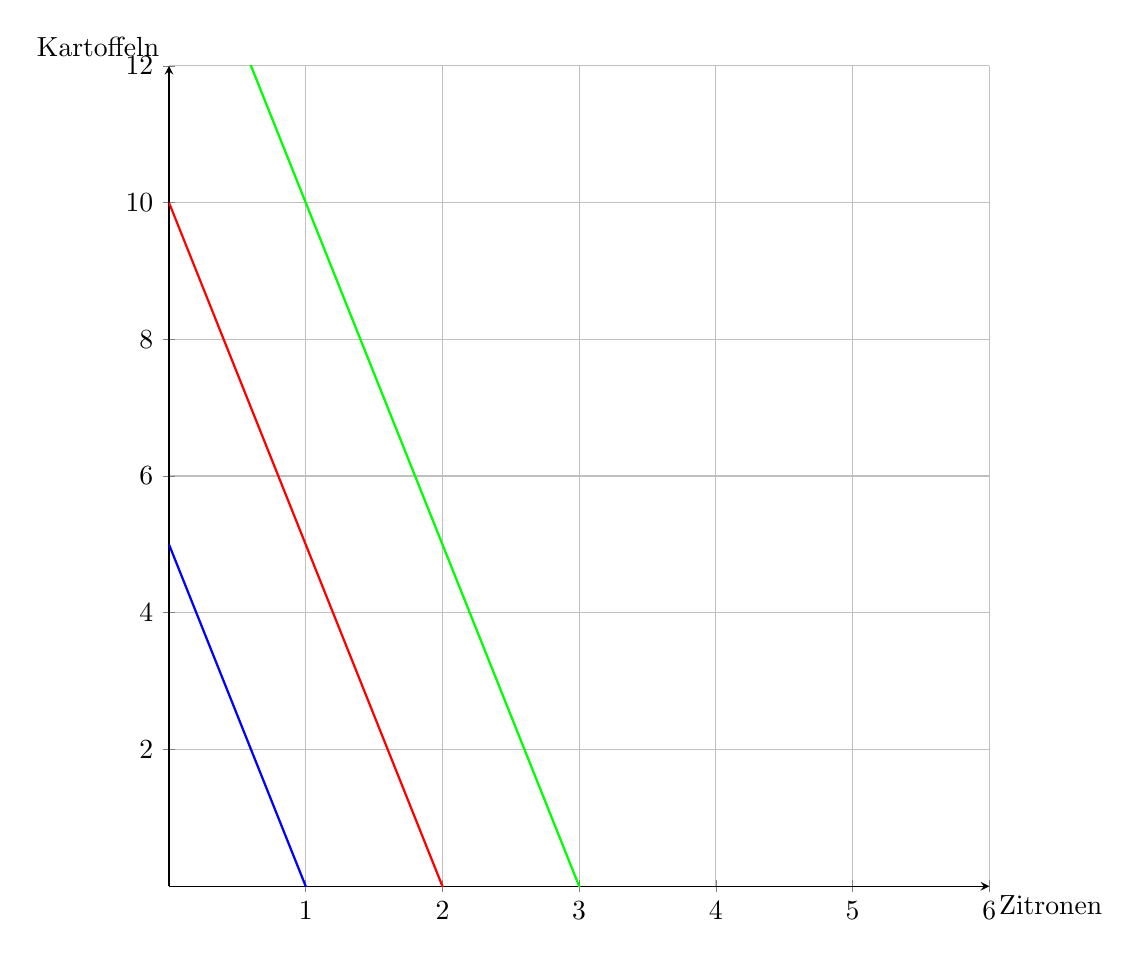
\begin{tikzpicture}
				      \begin{axis}[
						      axis lines=middle,
						      xlabel={Zitronen}, ylabel={Kartoffeln},
						      grid=both,
						      width=12cm, height=12cm,
						      xmin=0, xmax=6, ymin=0, ymax=12,
						      xtick={0,1,2,3,4,5,6},
						      ytick={0,2,4,6,8,10,12},
						      xlabel style={below right}, ylabel style={above left},
						      domain=0:6
					      ]

					      % Indifferenzkurve für C = 100
					      \addplot[thick,blue] {5 - 5*x};
					      %\node at (axis cs:3,5) [anchor=south east] {Indifferenzkurve für $C = 100$};

					      % Indifferenzkurve für C = 200
					      \addplot[thick,red] {10 - 5*x};
					      %\node at (axis cs:3,9) [anchor=south east] {Indifferenzkurve für $C = 200$};

					      % Indifferenzkurve für C = 300
					      \addplot[thick,green] {15 - 5*x};
					      %\node at (axis cs:3,11) [anchor=south east] {Indifferenzkurve für $C = 300$};

				      \end{axis}
			      \end{tikzpicture}

		      \end{center}

		\item Da nur Kaffe einen Einfluss hat, haben Papierservietten keinen Einfluss, weshalb vertikale Linien unsere Differenzkurve darstellen.
		      \begin{center}
			      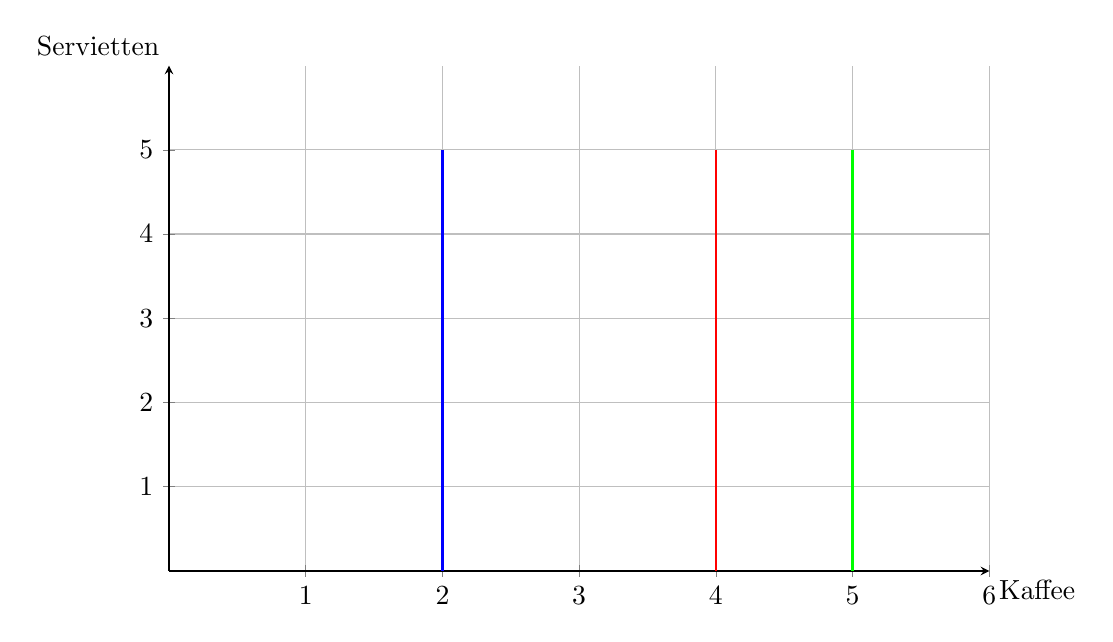
\begin{tikzpicture}
				      \begin{axis}[
						      axis lines=middle,
						      xlabel={Kaffee}, ylabel={Servietten},
						      grid=both,
						      width=12cm, height=8cm,
						      xmin=0, xmax=6, ymin=0, ymax=6,
						      xtick={0,1,2,3,4,5,6},
						      ytick={0,1,2,3,4,5},
						      xlabel style={below right}, ylabel style={above left},
						      domain=0:6
					      ]

					      % Indifferenzkurve für C = 100ml Kaffee (vertikale Linie)
					      \addplot[thick,blue] coordinates {(2,0) (2,5)}; % Beispiel: 100ml Kaffee, egal wie viele Servietten

					      % Indifferenzkurve für C = 200ml Kaffee (vertikale Linie)
					      \addplot[thick,red] coordinates {(4,0) (4,5)}; % Beispiel: 200ml Kaffee, egal wie viele Servietten

					      % Weitere Indifferenzkurve für 300ml Kaffee
					      \addplot[thick,green] coordinates {(5,0) (5,5)}; % Beispiel: 300ml Kaffee, egal wie viele Servietten

					      % Beschriftungen der Indifferenzkurven
					      %\node at (axis cs:2,5.5) [anchor=south east] {Indifferenzkurve für $100$ ml Kaffee};
					      %\node at (axis cs:4,5.5) [anchor=south east] {Indifferenzkurve für $200$ ml Kaffee};
					      %\node at (axis cs:5,5.5) [anchor=south east] {Indifferenzkurve für $300$ ml Kaffee};

				      \end{axis}
			      \end{tikzpicture}
		      \end{center}
		      Dies ist ein Beispiel für ein neutrales Gut.

		\item
		      Unsere Indiffernzkurven sind Linien, die sich rechtwinklig jeweils beim Verhältnis $9$ zu $1$ treffen.

		      \begin{center}

			      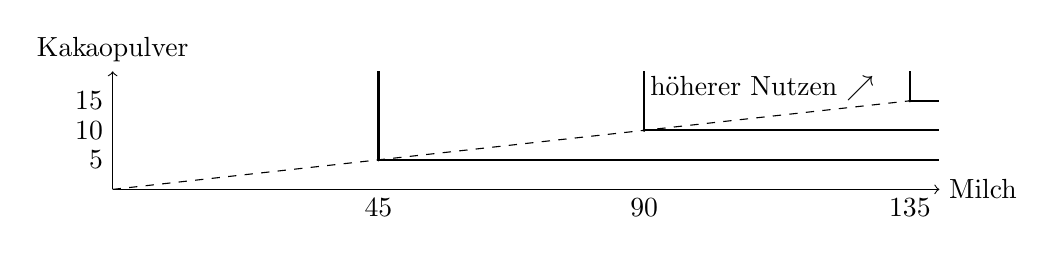
\begin{tikzpicture}[scale=0.075]

				      % Achsen
				      \draw[->] (0,0) -- (140,0) node[right] {Milch};
				      \draw[->] (0,0) -- (0,20) node[above] {Kakaopulver};

				      % Verhältnisslinie x2 = (1/9) x1
				      \draw[dashed, domain=0:135] plot (\x,{(1/9)*\x});%node[right] {$x_2 = \frac{1}{9}x_1$};

				      \draw[thick] (45,20) -- (45,5) -- (140,5);
				      \draw[thick] (90,20) -- (90,10) -- (140,10);
				      \draw[thick] (135,20) -- (135,15) -- (140,15);

				      \filldraw (45,5) circle (4pt);
				      \filldraw (90,10) circle (4pt);
				      \filldraw (135,15) circle (4pt);

				      % Beschriftung Indifferenzkurven
				      \node at (110,17) {höherer Nutzen $\nearrow$ };
				      % Beschriftung der Ecken
				      \node[below] at (45,0) {$45$};
				      \node[left] at (0,5) {$5$};
				      \node[below] at (90,0) {$90$};
				      \node[left] at (0,10) {$10$};
				      \node[below] at (135,0) {$135$};
				      \node[left] at (0,15) {$15$};

			      \end{tikzpicture}

		      \end{center}

	\end{enumerate}
\end{solution}


\begin{question}
	Kann eine Indifferenzkurve einer Konsumentin mit monotoner Präfernz wie folgt aussehen:

	\begin{center}
		\begin{tikzpicture}
			% Achsen zeichnen
			\draw[->] (0,0) -- (4,0) node[right] {$x_1$}; % x1-Achse
			\draw[->] (0,0) -- (0,4) node[above] {$x_2$}; % x2-Achse

			% Kreis zeichnen
			\draw[thick] (2,2) circle(1); % Kreis mit Radius 3

			% Beschriftung für den Kreis
			\node at (2,2) {$U$}; % Beispielhafte Beschriftung des Kreises (kann angepasst werden)

			% Markierung auf den Achsen
		\end{tikzpicture}
	\end{center}
	Erklären Sie Ihre Antwort. Wie verändert sich Ihre Antwort, wenn man auf die Annahme verzichtet,
	dass die Präferenz monoton ist?
\end{question}

\begin{solution}
	Nein, da monotone Präferenz verletzt wird, da die untere Kreishälfte jeweils auf der oberen Kreishälfte ein besseres gut mit mehr von beidem hat. Ist die Monotonieannahme nicht gegeben, kann die Indifferenzkurve so aussehen.
\end{solution}

\begin{question}
	Wird in der mikroökonomischen Theorie automatisch angenommen, dass Akteure egoistisch sind, wenn
	ihre Vorlieben mithilfe von Präferenzen modelliert werden? Begründen Sie Ihre Antwort.
\end{question}
\begin{solution}
	Nein, eine Präferenz sagt nichts über Egoismus aus. Beispielsweise können auch Gruppenpräferenzen modelliert werden, die nicht egosistisch sein können per Definition.
\end{solution}


\section{Blatt 2}

\begin{question}
	Finde eine Nutzenfunktion zur folgender Grafik:
	\begin{center}

		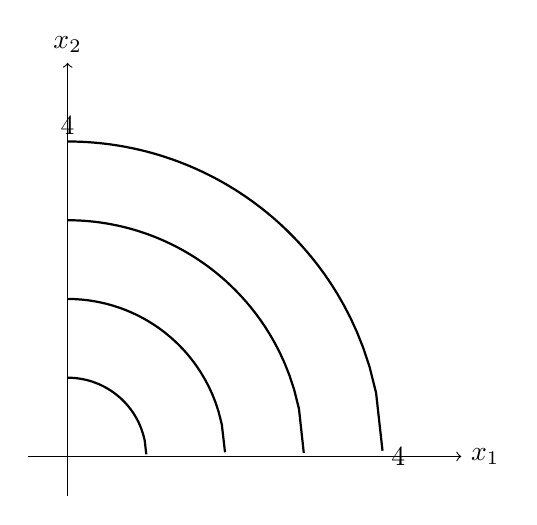
\begin{tikzpicture}
			% Achsen zeichnen
			\draw[->] (-0.5,0) -- (5,0) node[right] {$x_1$}; % x1-Achse
			\draw[->] (0,-0.5) -- (0,5) node[above] {$x_2$}; % x2-Achse

			% Viertelkreis mit Radius 1
			\draw[thick,domain=0:1,samples=50]
			plot (\x, {sqrt(1-\x^2)});
			%node[right] {$U_1$};

			% Viertelkreis mit Radius 2
			\draw[thick,domain=0:2,samples=50]
			plot (\x, {sqrt(4-\x^2)});
			%node[right] {$U_2$};

			% Viertelkreis mit Radius 3
			\draw[thick,domain=0:3,samples=50]
			plot (\x, {sqrt(9-\x^2)});
			%node[right] {$U_3$};

			% Viertelkreis mit Radius 4
			\draw[thick,domain=0:4,samples=50]
			plot (\x, {sqrt(16-\x^2)});
			%node[right] {$U_4$};

			% Markierungen auf den Achsen
			\node at (4.2, 0) {$4$};
			\node at (0, 4.2) {$4$};
		\end{tikzpicture}
	\end{center}
\end{question}
\begin{solution}
	Es handelt sich hierbei offensichtlich um die Kreisgleichung:
	\[
		u(x_1,x_2) = x_1^2+x_2^2 = c
		,\]
	wobei $x_i \ge 0$.
\end{solution}

\begin{question}
	Verschiedene Nutzenfunktionen können dieselben Präferenzen beschreiben. Welche der folgenden Nutzenfunktionen beschreiben Cobb-Douglas-Präferenzen?
	\begin{enumerate}
		\item  \( u(x_1, x_2) = x_1^{\frac{1}{3}} x_2^{\frac{2}{3}} -65 \)
		\item \( u(x_1, x_2) = x_1^5 \cdot x_2^4 \)
		\item  \( u(x_1, x_2) = \frac{1}{3} \ln x_1 + \frac{2}{3} \ln x_2 \)
		\item \( u(x_1, x_2) = \left( 2 \ln x_1 + 3 \ln x_2 + 111 \right)^3 \)
	\end{enumerate}
\end{question}
\begin{solution}
	\begin{enumerate}
		\item Es handelt sich um eine Verschiebung, weshalb die Präferenzordnung beibehalten wird.
		\item Wir können die Funktion
		\item Wir wissen, dass $5 + (1-5) = 9$ ist, also ist die zugrundeliegende Cobb-Douglas-Funktion:
		      \[
			      x_1^{\frac{5}{9}} \cdot x_2^{\frac{4}{9}}
			      .\]
		\item Wir verwenden die Eigenschaften des $\log$ und erhalten so:
		      \[
			      \frac{1}{3} \ln x_1 + \frac{2}{3} \ln x_2 = \ln x_1^{\frac{1}{3}}+ \ln x_2^{\frac{2}{3}} = \ln \left( x_1^{\frac{1}{3}} \cdot x_2^{\frac{2}{2}} \right)
			      .\]
		      Da $\ln$ eine streng monoton wachsende Funktion ist, handelt es sich um eine Cobb-Douglas-Präferenz.

		\item Kombiniere vorherige Lösungen und erhalte gleiches Resultat.
	\end{enumerate}
\end{solution}

\begin{question}[subtitle=Budgetmengen]
	\begin{enumerate}
		\item Anna verfügt über ein Einkommen von $m= 10$. Sie kann Gut 1 $(x_1)$ zum Preis $p_1 = 2$ und Gut 2
		      $(x_2)$ zum Preis $p_2 = 1$ kaufen. Zeichnen Sie Annas Budgetmenge in ein Koordinatensystem.
		\item Der Preis von Gut 2 steigt auf $p_2 = 2$, alle anderen Werte bleiben gleich. Zeichnen Sie die
		      neue Budgetmenge in dieselbe Grafik ein.
		\item Annas Einkommen steigt nun auf $m = 14$. Die Preise entsprechen weiterhin den geänderten Preisen.
		      Zeichnen Sie auch diese neue Budgetmenge in dieselbe Grafik ein.
		\item Kehren Sie zur Ausgangssituation aus Teil zurück. Wegen einer Knappheit beschließt die Regierung, dass maximal 3 Einheiten von Gut 1 pro Konsument verkauft werden dürfen. Zeichnen Sie die  entsprechende Budgetmenge in eine neue Grafik.
	\end{enumerate}
\end{question}

\begin{solution}
	\begin{enumerate}
		\item Unsere Budgetgerade ist: $2\cdot x_1 +x_2=10$:
		      \begin{center}

			      \begin{tikzpicture}
				      % Achsen zeichnen
				      \draw[->] (0,0) -- (6,0) node[right] {$x_1$}; % x1-Achse
				      \draw[->] (0,0) -- (0,12) node[above] {$x_2$}; % x2-Achse

				      % Budgetgerade zeichnen (x2 = 10 - 2*x1)
				      \draw[thick] (0,10) -- (5,0);

				      % Markierungen auf den Achsen
				      \node at (5.2, -0.5) {$5$};
				      \node at (-0.5, 10.2) {$10$};

				      % Beschriftung der Budgetgeraden
				      %\node at (2.5, 3) {Budgetgerade};

				      % Punkt (0,10) und (5,0)
				      \fill (0,10) circle (2pt);
				      %\node at (-0.3, 10) {$(0, 10)$};
				      \fill (5,0) circle (2pt);
				      %\node at (5, -0.3) {$(5, 0)$};
			      \end{tikzpicture}

		      \end{center}
		\item Wir machen es gleich:

		      \begin{center}

			      \begin{tikzpicture}
				      % Achsen zeichnen
				      \draw[->] (0,0) -- (6,0) node[right] {$x_1$}; % x1-Achse
				      \draw[->] (0,0) -- (0,12) node[above] {$x_2$}; % x2-Achse

				      % Alte Budgetgerade (p2 = 1) zeichnen (x2 = 10 - 2*x1)
				      \draw[thick, blue] (0,10) -- (5,0);
				      %\node at (2.5, 3) {Budgetgerade $p_2 = 1$};

				      % Neue Budgetgerade (p2 = 2) zeichnen (x2 = 5 - x1)
				      \draw[thick, red] (0,5) -- (5,0);
				      %\node at (2.5, 1) {Budgetgerade $p_2 = 2$};

				      % Markierungen auf den Achsen
				      \node at (5.2, -0.5) {$5$};
				      \node at (-0.5, 10.2) {$10$};
				      \node at (-0.5, 5.2) {$5$};

				      % Punktmarkierungen
				      \fill (0,10) circle (2pt);
				      %\node at (-0.3, 10) {$(0, 10)$};
				      \fill (5,0) circle (2pt);
				      %\node at (5, -0.3) {$(5, 0)$};

				      \fill (0,5) circle (2pt);
				      %\node at (-0.3, 5) {$(0, 5)$};

			      \end{tikzpicture}


		      \end{center}
		\item Nochmals:

		      \begin{center}

			      \begin{tikzpicture}
				      % Achsen zeichnen
				      \draw[->] (0,0) -- (8,0) node[right] {$x_1$}; % x1-Achse
				      \draw[->] (0,0) -- (0,12) node[above] {$x_2$}; % x2-Achse

				      % Alte Budgetgerade (p2 = 1) zeichnen (x2 = 10 - 2*x1)
				      \draw[thick, blue] (0,10) -- (5,0);
				      %				      \node at (2.5, 3) {Budgetgerade $p_2 = 1$};

				      % Neue Budgetgerade (p2 = 2) zeichnen (x2 = 5 - x1)
				      \draw[thick, red] (0,5) -- (5,0);
				      %				      \node at (2.5, 1) {Budgetgerade $p_2 = 2$};

				      % Budgetgerade nach Einkommenserhöhung (m = 14, p2 = 2) (x2 = 7 - x1)
				      \draw[thick, green] (0,7) -- (7,0);
				      %\node at (3.5, 3) {Budgetgerade $m = 14$};

				      % Markierungen auf den Achsen
				      \node at (5.2, -0.5) {$5$};
				      \node at (-0.5, 10.2) {$10$};
				      \node at (-0.5, 5.2) {$5$};
				      \node at (-0.5, 7.2) {$7$};

				      % Punktmarkierungen für die Budgetgeraden
				      \fill (0,10) circle (2pt);
				      %				      \node at (-0.3, 10) {$(0, 10)$};
				      \fill (5,0) circle (2pt);
				      %				      \node at (5, -0.3) {$(5, 0)$};

				      \fill (0,5) circle (2pt);
				      %				      \node at (-0.3, 5) {$(0, 5)$};

				      \fill (0,7) circle (2pt);
				      %				      \node at (-0.3, 7) {$(0, 7)$};

				      \fill (7,0) circle (2pt);
				      %				      \node at (7, -0.3) {$(7, 0)$};

			      \end{tikzpicture}


		      \end{center}

		\item Nun die Beschränkung:

		      \begin{center}

			      \begin{tikzpicture}
				      % Achsen zeichnen
				      \draw[->] (0,0) -- (6,0) node[right] {$x_1$}; % x1-Achse
				      \draw[->] (0,0) -- (0,12) node[above] {$x_2$}; % x2-Achse

				      % Budgetgerade (p2 = 1) zeichnen (x2 = 10 - 2*x1) bis x1 = 3
				      \draw[thick, blue] (0,10) -- (3,4);

				      % Horizontale Linie ab x1 = 3, x2 = 4
				      \draw[thick, blue] (3,4) -- (3,0);

				      % Markierungen auf den Achsen
				      \node at (3.2, -0.5) {$3$};
				      \node at (5.2, -0.5) {$5$};
				      \node at (-0.5, 10.2) {$10$};
				      \node at (-0.5, 4.2) {$4$};

				      % Punktmarkierungen
				      \fill (0,10) circle (2pt);
				      % \node at (-0.3, 10) {$(0, 10)$};
				      \fill (3,4) circle (2pt);
				      \node at (3.5, 4.2) {$(3, 4)$};
				      \fill (5,0) circle (2pt);
				      % \node at (5, -0.3) {$(5, 0)$};

				      % Beschriftung der Budgetmenge
				      %				      \node at (1.5, 7) {Budgetmenge mit Obergrenze};

			      \end{tikzpicture}

		      \end{center}
	\end{enumerate}

\end{solution}

\begin{question}[subtitle={Cobb-Douglas-Präferenzen}]
	Wir betrachten die Nutzenfunktion
	\[
		u(x_1,x_2) = x_1^{\frac{1}{3}} x_2^{\frac{2}{3}}
		.\]
	Dabei bezeichnet $x_1$ die Ausgaben in Euro für Nahverkehr, und $x_2$ die Ausgaben in Euro für
	alle anderen Konsumgüter.
	\begin{enumerate}
		\item Bestimmen Sie die optimale Entscheidung des Haushalts in Abhängigkeit vom Einkommen $m$\footnote{Beide Güter haben per Definition einen Preis von 1 Euro, da $x_1$ und $x_2$ direkt Ausgaben darstellen}.
		\item Der Staat führt einen Mobilitätszuschuss ein und übernimmt 50 \% der Ausgaben für Nahverkehr.
		      Die Subvention wird aus Steuermitteln finanziert, sodass der Konsument nun für 50 Cent Nahverkehrsgüter im Wert von 1 Euro erhält. Wie verändert sich die Budgetmenge?
		      Wie verändert sich die optimale Entscheidung?
		\item Berechnen Sie den Subventionsbetrag aus dem Aufgabenteil davor, der aus Steuermitteln finanziert wird.
		      Wäre der Haushalt besser gestellt, wenn der Staat statt der Subvention eine gleich hohe Barzahlung leisten würde? Sie können diese Frage beantworten, indem Sie entweder grafisch argumentieren oder berechnen, welches Konsumbündel der Haushalt wählen würde, wenn er den Subventionsbetrag als Barzahlung erhielte – und anschließend prüfen, ob dieses Bündel einen höheren Nutzen liefert als das
		      im zuvor Berechneten.
	\end{enumerate}
\end{question}

\begin{solution}
	\begin{enumerate}
		\item Wir stellen unsere Lagrange-Funktion auf:
		      \[
			      \mathcal{L}(x_1, x_2, \lambda) = x_1^{\frac{1}{3}} x_2^{\frac{2}{3}}  + \lambda (m -x_1 -x_2)
			      .\]
		      Nun bilden wir unsere Bedingungen erster Ordnung:
		      \begin{align}
			      \frac{\partial \mathcal{L}}{\partial x_1}     & = \frac{1}{3} x_1^{-\frac{2}{3}} x_2^{\frac{2}{3}} - \lambda \label{eq:solution1} \\
			      \frac{\partial \mathcal{L}}{\partial x_2}     & = \frac{2}{3} x_1^{\frac{1}{3}} x_2^{-\frac{1}{3}} - \lambda \label{eq:solution2} \\
			      \frac{\partial \mathcal{L}}{\partial \lambda} & = m-x_1-x_2
			      .\end{align}
		      Nun müssen wir die Bedingungen $0$ setzen und das resultierende Gleichungssystem lösen. Dazu setzten wir \eqref{eq:solution1} und \eqref{eq:solution2} gleich:
		      \begin{align*}
			      \frac{1}{3} \left(\frac{x_2}{x_1} \right)^{\frac{2}{3}} = \frac{2}{3} \left( \frac{x_1}{x_2} \right)^{\frac{1}{3}} & \iff \left( \frac{x_2}{x_1} \right)^{\frac{2}{3}} = 2\cdot  \left( \frac{x_1}{x_2} \right)^{\frac{1}{3}}
			      .\end{align*}
		      Umformungen und einsetzen in die Nebenbedingung liefert:
		      \begin{align}
			      x_1^* = \frac{m}{3}, \qquad x_2^* =  \frac{2}{3} m
		      \end{align}

		\item Die Nebenbedingung für $x_1$ bleibt unverändert, so auch $x_1^*$ $x_2^*$ verändert sich auf $\frac{2}{3} m$. Also gilt:
		      \[
			      x_1^* = x_2^* = \frac{2}{3} m
			      .\]
		\item Die Staatlichen Subventionen betragen
		      \[
			      \frac{2}{3}m - \frac{m}{3} = \frac{m}{3}
			      .\]
		      Die neue Beschränkung der Budgetmenge ist nun:
		      \[
			      m_{\operatorname{new}} = m+ \frac{m}{3} = \frac{4}{3} m
			      .\]
		      Daraus resultieren unsere neuen Optima:
		      \[
			      x_1^* = \frac{4}{9} m \qquad x_2^* = \frac{8}{9} m
			      .\]
		      Einsetzen in die Nutzenfunktion zeigt, dass die Barzahlung zu einem höheren Nutzen führt.
	\end{enumerate}
\end{solution}


\begin{question}[subtitle={Perfekte Komplemente}]
	Ein Konsument hat die Nutzenfunktion: $u(x_1, x_2) = \min(x_1, 3x_2)$.
	Der Konsument verfügt über ein Budget von $m= 8$ Euro.
	Der Preis $p_1$ für Gut 1 beträgt $1$ Euro, und der Preis $p_2$ für Gut 2 ebenfalls $1$ Euro
	\begin{enumerate}
		\item Zeichnen Sie die Budgetmenge und skizieren Sie einige Indifferenzkurven. Können Sie das optimale
		      Bündel für den Konsumenten bestimmen?
		\item Nehmen Sie an, der Preis $p_1$ fürr Gut 1 veröndert sich. Können Sie die Nachfrage des Konsumenten
		      als Funktion des Preises $p_1$  bestimmen?
	\end{enumerate}
\end{question}

\begin{solution}
	\begin{enumerate}
		\item Das optimale Verhältnis der Mengen ist:
		      \[
			      x_1 = 3x_2 \iff \frac{x_1}{x_2} = 3
			      .\]
		      Im Optimum muss der Konsument dreimal soviel von Gut 1 wie von Gut 2 konsumieren.
		      Die Eckpunkte der Indifferenzkurven liegen also bei $(3,1), (6,2), (9,3)$, und so weiter.
		      Wir visualisieren nun die Indifferenzkurzen (in rot) und die Budgetgerade (in blau):
		      \begin{center}

			      \begin{tikzpicture}[scale=0.8]
				      % Achsen
				      \draw[->] (0,0) -- (10,0) node[right] {$x_1$};
				      \draw[->] (0,0) -- (0,10) node[above] {$x_2$};

				      % Budgetgerade
				      \draw[blue, thick] (0,8) -- (8,0);

				      % Indifferenzkurven (L-förmig, Ecke am optimalen Punkt)
				      \draw[red, thick] (6,2) -- (6,8); % vertikal ab optimalem Punkt nach oben
				      \draw[red, thick] (6,2) -- (9,2); % horizontal ab optimalem Punkt nach rechts

				      \draw[red, thick] (3,1) -- (3,6); % zweite Kurve: vertikal
				      \draw[red, thick] (3,1) -- (7,1); % zweite Kurve: horizontal

				      % Optimales Bündel
				      \filldraw[black] (6,2) circle (2pt);

				      % Achsenbeschriftung
				      \foreach \x in {3,6,8}
				      \draw (\x,0) -- (\x,-0.2) node[below] {\x};

				      \foreach \y in {1,2,8}
				      \draw (0,\y) -- (-0.2,\y) node[left] {\y};

			      \end{tikzpicture}
		      \end{center}
		      Das optimale Bündel ist demnach: $(x_1^*,x_2^*) = (6,2)$.
		\item Im Optimum muss gelten, dass $x_1 = 3x_2$. Einsetzen in die Budgetgerade liefert und:
		      \[
			      p_1(3x_2^*) + x_2^* = 8 \iff (3p_1+1)x_2^* = 8  \iff x_2^* = \frac{8}{3p_1+1}
			      .\]
		      Also gilt für $x_1^* = \frac{24}{3p_1+1}$.
	\end{enumerate}
\end{solution}

\section{Blatt 3}


\begin{question}
	Ein Haushalt konsumiert zwei Güter und maximiert die Nutzenfunktion:
	\[
		u(x_1,x_2) = x_1 \cdot x_2^2
		.\]
	\begin{enumerate}
		\item Bestimmen Sie die Nachfrage als Funktion des Einkommens $m$ sowie der Preise $p_1$ und $p_2$. Was
		      wird nachgefragt, wenn das Einkommen 9 Euro beträgt und beide Preise jeweils 1 Euro sind?
		\item  Nehmen Sie an, der Preis für Gut 1 steigt von 1 Euro auf 2 Euro. Bestimmen den Einkommens-
		      und den Substitutionseffekt für diese Preisänderung.
		\item Nehmen Sie an, der Preis für Gut 1 steigt von 1 Euro auf 2 Euro. Bestimme Einkommens-
		      und  Substitutionseffekt für diese Preisänderung.
		\item Wie ist das Vorzeichen des Substitutionseffekts? Könnte der Substitutionseffekt auch positiv sein?
		      Begründen Sie Ihre Antwort.
	\end{enumerate}
\end{question}
\begin{solution}

	\begin{enumerate}
		\item Wir lösen
		      \[
			      \max x_1 x_2^2 \qquad \text{u. d. NB } \quad p_1 x_1 + p_2 x_2 = m
			      .\]
		      Die Lagrange-Funktion ist:
		      \[
			      \mathcal{L}(x_1,x_2,\lambda) = x_1x_2^2 + \lambda \left( m - p_1 x_1 -p_2 x_2 \right)
			      .\]
		      Ableiten und Null setzen liefert uns:
		      \begin{align*}
			      \frac{\partial \mathcal{L}}{\partial x_1} & =  x_2^2 - \lambda p_1 = 0    \\
			      \frac{\partial \mathcal{L}}{\partial x_2} & =  2x_1x_2 - \lambda p_2 = 0.
		      \end{align*}
		      Umstellen ergibt und gleichsetzen liefert uns:
		      \[
			      \frac{x_2^2}{p_1} = \frac{2x_1x_2}{p_2} \iff x_2 = \frac{2 p_1}{p_2}x_1
			      ,\]
		      wobei $x_2 \neq 0$  sein muss.
		      Einsetzen in die Nebenbedingung (bzw. die Ableitung nach $\lambda$) ergibt:
		      \[
			      p_1 x_1 + p_2 \left( \frac{2p_1}{p_2}x_1 \right) =m
			      .\]
		      Daraus resultiert direkt:
		      \[
			      x_1^* = \frac{m}{3p_1} , \qquad \text{ und } \qquad x_2^* = \frac{2}{3} \frac{m}{p_2}
			      .\]
		      Demnach wird für $m=9$ und $p_i = 1$ folgendes Bündel nachgefragt:
		      \[
			      (x_1^*,x_2^*) = (3,6)
			      .\]
		\item Wir bestimmen zu erst den Gesamteffekt: $x_1(p_1',p_2,m) - x_1(p_1,p_2,m)$:
		      \[
			      \frac{9}{3\cdot 2} - \frac{9}{3} = 1.5 - 3=  -1.5
			      .\]
		      Wir müssen nun noch $\Delta m$ berechnen, um $x_1(p_1',p_2,m + \Delta m)$ zu bestimmen.
		      Es ist:
		      \[
			      \Delta m = x_1 \cdot \Delta p = 3 \cdot (2-1) = 3
			      .\]
		      Nun können wir bestimmen:
		      \[
			      x_1(p_1',p_2,m')= \frac{12}{6} = 2
			      .\]
		      Demnach erhalten wir:
		      \[
			      \operatorname{SE} = 2 - 3 = -1
			      .\]
		      Der Einkommenseffekt ergibt sich folglich:
		      \[
			      \operatorname{EE} =  1.5 - 2 = -0.5
			      .\]
		\item Der Einkommenseffekt ist negativ. Steigt $p_1$, so sinkt die Nachfrage nach $x_1$
		\item Das Vorzeichen des Subsitutionseffekt kann nicht positiv sein. Wenn $p_1$ steigt und das Einkommen kompensiert wird, wird auch weniger $x_1$ nachgefragt.
	\end{enumerate}

\end{solution}


\begin{question}[subtitle={Aggregierte Nachfrage, Elastizitäten und Konsumentenrente}]
	Stellen Sie sich eine Konsumentin vor, die  für ihre Mahlzeiten gerne Käse ($x_1$) und Brot ($x_2$) kombiniert.
	Für eine ausgewogene Mahlzeit konsumiert sie die beiden Güter stets im Verhältnis 2:1 (z. B. 2 Scheiben
	Käse und 1 Scheibe Brot). Zusätzliche Einheiten von Käse oder Brot, die nicht in diesem Verhältnis
	konsumiert werden kännen, sind für sie nutzlos (z. B. 3 Scheiben Käase und 1 Scheibe Brot sind für sie
	genauso gut wie 2 Scheiben Käse und 1 Scheibe Brot).
	Der Preis von Käse beträgt $p$ Euro pro Scheibe, der Preis von Brot ist 1 Euro pro Scheibe. Das
	monatliche Budget der Konsumentin beträgt 60 Euro.
	\begin{enumerate}
		\item Bestimmen Sie die Nachfrage der Konsumentin für Käse in Abhängigkeit vom Preis $p$.
		\item Berechne die Preiselaszität. Welche Elaszität hat die Nachfrage bei einem Preis von $p=1$?
		\item Bestimme die aggregierte Nachfragefunktion für $20$ identische Konsumenten.
	\end{enumerate}
\end{question}

\begin{solution}

	\begin{enumerate}
		\item Wir setzen $x_1 = 2x_2$ in die Budgetrestriktion ein:
		      \[
			      p_2x_2 + x_2 = 60 \implies x_2 = \frac{60}{2p_1}, \text{ und } x_1 = \frac{120}{2p+1}
			      .\]
		\item Es gilt:
		      \[
			      \epsilon_D = \frac{d x_1}{d p} \cdot \frac{p}{x_1} = \frac{-240}{(2p+1)^2} \cdot \frac{p(2p+1)}{120} = \frac{2p}{2p+1}
			      .\]
		      Für $p=1$ gilt:
		      \[
			      \epsilon_D(1) = \frac{2}{2+1} = \frac{2}{3}
			      .\]
		\item Wir haben die Nachfragefunktionen der einzelen Konsumenten bereits errechnet. Da diese identisch sind, müssen wir diese nur noch summieren.
		      Die Anwendung des Distributivgesetzt liefert und dann direkt:
		      \[
			      20 \cdot \frac{120}{2p+1} = \frac{2400}{2p+1}\quad \& \quad 20\cdot \frac{60}{2p_1} = \frac{1200}{2p_1}
			      .\]
	\end{enumerate}
\end{solution}

\begin{question}
	Eine Studentin hat in dieser Klausurperiode noch zwei Prüfungen: Makro und Mikro. Sie überlegt,
	wie sie die insgesamt 9 verbleibenden Stunden zur Vorbereitung optimal auf die beiden Fächer verteilen soll.
	Sie geht davon aus, dass sich ihre Note in einem Fach allein durch die investierte Lernzeit wie folgt
	ergibt:
	\begin{itemize}
		\item

	\end{itemize}
\end{question}


\section{Blatt 4}

\begin{question}

	Die Präferenzen einer Konsumentin werden durch die Nutzenfunktion
	\[
		u(C,F) = \frac{1}{4} C +8 \ln(F)
	\]
	beschrieben, wobei $C$ der Konsum und $F$ die Freizeit darstellt.
	Es gilt:
	\[
		F+L = 12
		,\]
	wobei $L$ die geleistete Arbeit ist. Sie erhält einen Lohn $w$, das heißt es gilt:
	\[
		C = w \cdot L
		.\]
	\begin{enumerate}
		\item Formuliere das Maximierungsproblem und berechne den optimalen Konsum, wenn $w=12$ ist. .
		\item Angenommen, durch eine Steuererhöhung sinkt das Nettogehalt der Konsumentin auf
		      $10$ Euro. Berechnen Sie, wie sich die optimale Arbeitszeit verändert, wenn sich die Konsumentin anpasst. Interpretieren Sie das Ergebnis.
	\end{enumerate}
\end{question}

\begin{solution}

	\begin{enumerate}
		\item Wir setzen die Nebenbedingungen ein und erhalten so:
		      \[
			      \max_{F \in (0,12)} u(F) = 3w- \frac{1}{4} w F + \ln(F)
			      .\]
		      Bilden wir nun die Bedingung erster Ordnung erhalten wir:
		      \[
			      \frac{\mathrm{d} u}{\mathrm{d} F} = -3 + \frac{8}{F}
			      .\]
		      Nullsetzen ergibt: $F^* = \frac{8}{3}$. Einsetzen ergibt:
		      \begin{align*}
			      L^* = 12 - F^* & = 12 - \frac{8}{3} = \frac{28}{3} \\
			      C^*            & = 12* L^* = 112
			      .\end{align*}
		\item Wir kennen bereits die optimale Enscheidung. Einsetzen liefert:
		      \[
			      F^* = \frac{8}{2.5} = 3.2 \qquad \& \qquad L^* = 8.8
			      .\]
		      Wir bemerken, dass der Subsitutionseffekt die Arbeitszeit nach unten zieht und der Einkommenseffekt dies nicht dominiert.
	\end{enumerate}
\end{solution}

\section{Blatt 5}

\begin{question}
	Ein preisnehmendes Unternehmen produziert K-Phones. Die Produktionsfunktion ist gegeben durch:
	\[
		f(K, L) = K^{1/3} L^{1/2}
	\]
	Angenommen, das Kapital \(K\) ist kurzfristig fix auf \(K_0 = 1\) und kann nicht verändert werden. Bezeichnen Sie mit \(r\) bzw. \(w\) die Preise für Kapital und Arbeit. Der Marktpreis eines K-Phones sei \(p\). Die Preise seien gegeben durch \(p = 5\), \(r = 1\) und \(w = 1\).

	\begin{enumerate}
		\item Bestimmen Sie die optimale Wahl des Arbeitseinsatzes in der kurzen Frist. Welchen Gewinn erzielt das Unternehmen?
		\item Bestimmen Sie die optimale Wahl von Arbeit und Kapital in der langen Frist. Welchen Gewinn erzielt das Unternehmen?
		\item Vergleichen Sie die Gewinne aus Teil (a) und (b). Erklären Sie, warum sie sich unterscheiden.
		\item Kann es für einige Preisniveaus \(r, w\) und \(p\) vorkommen, dass das Unternehmen in der langen Frist einen positiven Gewinn erzielt, der dem kurzfristigen Gewinn entspricht?
	\end{enumerate}
\end{question}

\begin{solution}
	\begin{enumerate}
		\item \textbf{Kurze Frist:}
		      Produktionsfunktion:
		      \[
			      f(1, L) = L^{1/2}
		      \]
		      Gewinnfunktion:
		      \[
			      \Pi(L) = 5 \cdot L^{1/2} - 1 \cdot L - 1
		      \]
		      Gewinnmaximierung:
		      \[
			      \frac{d\Pi}{dL} = \frac{5}{2} L^{-1/2} - 1 = 0
		      \]
		      \[
			      L^* = \left(\frac{5}{2}\right)^2 = 6.25
		      \]
		      Gewinn:
		      \[
			      \Pi(6.25) = 5 \cdot \sqrt{6.25} - 6.25 - 1 = 12.5 - 7.25 = 5.25
		      \]
		      Der Gewinn in der kurzen Frist beträgt also \(\boxed{5.25}\).

		\item \textbf{Lange Frist:} (Neu machen, irgendwie bisschen sketchy von mir)
		      Produktionsfunktion:
		      \[
			      f(K, L) = K^{1/3} L^{1/2}
		      \]
		      Kosten:
		      \[
			      C = rK + wL = K + L
		      \]
		      Kostenminimale Faktorkombination:
		      \[
			      \frac{MP_K}{r} = \frac{MP_L}{w}
		      \]
		      Grenzprodukte:
		      \[
			      MP_K = \frac{1}{3} K^{-2/3} L^{1/2}, \quad MP_L = \frac{1}{2} K^{1/3} L^{-1/2}
		      \]
		      Verhältnis:
		      \[
			      \frac{\frac{1}{3} K^{-2/3} L^{1/2}}{1} = \frac{\frac{1}{2} K^{1/3} L^{-1/2}}{1}
		      \]
		      Auflösen:
		      \[
			      L = \frac{3}{2} K
		      \]
		      In Produktionsfunktion einsetzen:
		      \[
			      q = K^{1/3} \left(\frac{3}{2} K\right)^{1/2} = \left(\frac{3}{2}\right)^{1/2} K^{5/6}
		      \]
		      Umstellen nach \(K\):
		      \[
			      K = \left(\frac{q}{\left(\frac{3}{2}\right)^{1/2}}\right)^{6/5}
		      \]
		      Gesamtkosten:
		      \[
			      C(q) = K + L = K + \frac{3}{2} K = \frac{5}{2} K
		      \]
		      Einsetzen:
		      \[
			      C(q) = \frac{5}{2} \left(\frac{q}{\left(\frac{3}{2}\right)^{1/2}}\right)^{6/5}
		      \]
		      Gewinn:
		      \[
			      \Pi(q) = 5q - C(q)
		      \]
		      Maximieren durch:
		      \[
			      \frac{d\Pi}{dq} = 5 - \frac{dC}{dq} = 0
		      \]
		      Mit:
		      \[
			      \frac{dC}{dq} = \frac{6}{5} \cdot \frac{5}{2} \cdot \left(\frac{1}{\left(\frac{3}{2}\right)^{1/2}}\right)^{6/5} \cdot q^{1/5}
		      \]
		      Gewinnmaximum bestimmen, ergibt einen höheren Gewinn als in der kurzen Frist, da das Unternehmen beide Faktoren optimal wählen kann.

		\item \textbf{Vergleich:}
		      In der langen Frist kann das Unternehmen beide Produktionsfaktoren anpassen und so die kostengünstigste Faktorkombination wählen. In der kurzen Frist ist das Kapital fix und das Unternehmen kann nur den Arbeitseinsatz optimieren. Daher ist der Gewinn in der langen Frist höher.

		\item \textbf{Möglichkeit identischen Gewinns:}
		      Ja, falls die Faktorpreise \(r, w\) so gewählt sind, dass die kostenminimale Faktorkombination in der langen Frist exakt der in der kurzen Frist entspricht (hier \(K=1, L=6.25\)). Dies ist allerdings nur bei bestimmten Preisverhältnissen der Fall und somit ein Spezialfall.
	\end{enumerate}

\end{solution}


\begin{question}
	Gegeben sei die Produktionsfunktion:
	\[
		f(K, L) = K^{\frac{1}{3}} \cdot L^{\frac{1}{3}}
	\]
	mit Faktorkosten \( r = 2 \) für Kapital und \( w = 1 \) für Arbeit.

	\begin{enumerate}
		\item Bestimmen Sie die Kostenfunktion.
		\item Bestimmen Sie, wie sich die Kostenfunktion verändert, wenn der Preis für Kapital von \( r = 2 \) auf \( r = 1 \) sinkt.
		\item Betrachten Sie den Fall \( r = 1 \). Der Produzent wählt \( y \), um den Gewinn zu maximieren, d.h.
		      \[
			      \max_{y} \, p \cdot y - c(y)
		      \]
		      wobei \( p = 6 \) der Preis des Outputgutes und \( c(y) \) die Kostenfunktion ist. Welche Menge \( y \) wird gewählt?
	\end{enumerate}

\end{question}
\begin{solution}
	\begin{enumerate}
		\item \textbf{Bestimmung der Kostenfunktion:}

		      Minimierungsproblem:
		      \[
			      \min_{K, L} \, C = 2K + 1 \cdot L
		      \]
		      mit Nebenbedingung:
		      \[
			      K^{\frac{1}{3}} L^{\frac{1}{3}} = y
		      \]

		      Lagrange-Funktion:
		      \[
			      \mathcal{L}(K, L, \lambda) = 2K + L + \lambda \left( y - K^{\frac{1}{3}} L^{\frac{1}{3}} \right)
		      \]

		      1. Ableitungen:
		      \[
			      \frac{\partial \mathcal{L}}{\partial K} = 2 - \lambda \cdot \frac{1}{3} K^{-\frac{2}{3}} L^{\frac{1}{3}} = 0
		      \]
		      \[
			      \frac{\partial \mathcal{L}}{\partial L} = 1 - \lambda \cdot \frac{1}{3} K^{\frac{1}{3}} L^{-\frac{2}{3}} = 0
		      \]
		      \[
			      \frac{\partial \mathcal{L}}{\partial \lambda} = y - K^{\frac{1}{3}} L^{\frac{1}{3}} = 0
		      \]

		      2. Verhältnis der Bedingungen:
		      \[
			      \frac{2}{1} = \frac{K^{-\frac{2}{3}} L^{\frac{1}{3}}}{K^{\frac{1}{3}} L^{-\frac{2}{3}}}
		      \]
		      \[
			      2 = \frac{L}{K}
		      \]
		      \[
			      L = 2K
		      \]

		      3. In Produktionsfunktion einsetzen:
		      \[
			      (K^{\frac{1}{3}} (2K)^{\frac{1}{3}}) = y
		      \]
		      \[
			      K^{\frac{2}{3}} \cdot 2^{\frac{1}{3}} = y
		      \]
		      \[
			      K = \left( \frac{y}{2^{\frac{1}{3}}} \right)^{\frac{3}{2}}
		      \]

		      4. Gesamtkosten:
		      \[
			      C(y) = 2K + L = 4K
		      \]
		      \[
			      C(y) = 4 \left( \frac{y}{2^{\frac{1}{3}}} \right)^{\frac{3}{2}}
		      \]
		      \[
			      = 2^{\frac{3}{2}} y^{\frac{3}{2}}
		      \]

		\item \textbf{Kostenfunktion bei \( r = 1 \):}

		      Verhältnis:
		      \[
			      \frac{1}{1} = \frac{L}{K}
		      \]
		      \[
			      L = K
		      \]

		      In Produktionsfunktion:
		      \[
			      (K^{\frac{1}{3}} K^{\frac{1}{3}}) = y
		      \]
		      \[
			      K^{\frac{2}{3}} = y
		      \]
		      \[
			      K = y^{\frac{3}{2}}
		      \]
		      \[
			      L = y^{\frac{3}{2}}
		      \]

		      Gesamtkosten:
		      \[
			      C(y) = K + L = 2 y^{\frac{3}{2}}
		      \]

		\item \textbf{Gewinnmaximierung:}

		      Gewinnfunktion:
		      \[
			      \Pi(y) = p \cdot y - C(y) = 6y - 2 y^{\frac{3}{2}}
		      \]

		      1. Ableitung:
		      \[
			      \frac{d \Pi}{dy} = 6 - 3 y^{\frac{1}{2}}
		      \]

		      Nullsetzen:
		      \[
			      6 - 3 y^{\frac{1}{2}} = 0
		      \]
		      \[
			      y^{\frac{1}{2}} = 2
		      \]
		      \[
			      y = 4
		      \]

		      \textbf{Ergebnis:} Die gewinnmaximierende Menge ist \( y = 4 \).

	\end{enumerate}

\end{solution}





\begin{question}
	Empirisch wurde beobachtet, dass in kurzen Rezessionen die durchschnittliche Arbeitsproduktivität – definiert als Output pro Arbeitsstunde – steigen kann.

	Um dies zu verstehen, betrachten Sie folgendes Setting:
	Ein Unternehmen produziert K-Phones mit der Produktionsfunktion:
	\[
		f(K, L) = K^{1/3} L^{1/2}
	\]
	Der Outputpreis beträgt zunächst \(p = 5\), die Inputpreise sind \(r = 1\) und \(w = 1\). Vor der Rezession wählt das Unternehmen Kapital und Arbeit optimal.

	Nun stellen Sie sich vor, dass der Outputpreis infolge einer Rezession plötzlich auf \(p = 1\) fällt.

	Unter der Annahme, dass das Kapital kurzfristig nicht angepasst werden kann (d.h. \(K\) bleibt auf dem Vorkrisenniveau), berechnen Sie:
	\begin{enumerate}
		\item Wie verändert sich die durchschnittliche Produktivität pro Stunde in der kurzen Frist?
		\item Steigt oder sinkt sie? Erklären Sie, warum dies geschieht.
	\end{enumerate}
\end{question}

\begin{solution}
	Hier ist irgendetwas falsch gelaufen?
	\begin{enumerate}
		\item Vor der Rezession wählt das Unternehmen die Faktormengen \(K\) und \(L\) optimal (vgl. lange Frist).

		      Nach der Rezession fällt der Outputpreis auf \(p = 1\).

		      In der kurzen Frist ist das Kapital fix (auf dem Vorkrisenniveau \(K_0\)), und das Unternehmen wird seinen Arbeitseinsatz neu optimieren.

		      Gewinnfunktion:
		      \[
			      \Pi(L) = p \cdot f(K_0, L) - w \cdot L - r \cdot K_0
		      \]
		      \[
			      = 1 \cdot K_0^{1/3} L^{1/2} - 1 \cdot L - r \cdot K_0
		      \]

		      Gewinnmaximierung:
		      \[
			      \frac{d\Pi}{dL} = \frac{1}{2} K_0^{1/3} L^{-1/2} - 1 = 0
		      \]
		      \[
			      L^*_{\text{neu}} = \left(\frac{1}{2} K_0^{1/3}\right)^2 = \frac{1}{4} K_0^{2/3}
		      \]

		      Durchschnittliche Produktivität nach der Rezession:
		      \[
			      \frac{f(K_0, L^*_{\text{neu}})}{L^*_{\text{neu}}}
			      = \frac{K_0^{1/3} (L^*_{\text{neu}})^{1/2}}{L^*_{\text{neu}}}
			      = K_0^{1/3} (L^*_{\text{neu}})^{-1/2}
		      \]
		      Einsetzen:
		      \[
			      = K_0^{1/3} \left(\frac{1}{4} K_0^{2/3}\right)^{-1/2}
			      = K_0^{1/3} \cdot 2 K_0^{-1/3}
			      = 2
		      \]

		      Vor der Rezession:
		      \[
			      L^*_{\text{vor}} = \left(\frac{5}{2} K_0^{1/3}\right)^2 = \frac{25}{4} K_0^{2/3}
		      \]
		      Durchschnittliche Produktivität:
		      \[
			      \frac{f(K_0, L^*_{\text{vor}})}{L^*_{\text{vor}}}
			      = \frac{K_0^{1/3} (L^*_{\text{vor}})^{1/2}}{L^*_{\text{vor}}}
			      = K_0^{1/3} (L^*_{\text{vor}})^{-1/2}
		      \]
		      Einsetzen:
		      \[
			      = K_0^{1/3} \left(\frac{25}{4} K_0^{2/3}\right)^{-1/2}
			      = K_0^{1/3} \cdot \frac{2}{5} K_0^{-1/3}
			      = \frac{2}{5}
		      \]

		\item \textbf{Vergleich:}
		      Vor der Rezession: \(\frac{2}{5} = 0.4\)
		      Nach der Rezession: \(2.0\)

		      Die durchschnittliche Produktivität pro Stunde steigt in der kurzen Frist deutlich.

		      \textbf{Begründung:}
		      Bei gesunkenem Outputpreis wird der Arbeitseinsatz stark reduziert, da sich die zusätzliche Produktion nicht mehr lohnt. Da aber das Kapital kurzfristig fix ist und der verbleibende Arbeitseinsatz geringer wird, entfällt der Output auf weniger Arbeitsstunden. Dadurch steigt der Output pro verbleibender Arbeitsstunde.

		      Dies erklärt das empirische Phänomen, dass in kurzen Rezessionen die durchschnittliche Produktivität pro Stunde ansteigen kann.
	\end{enumerate}
\end{solution}




\clearpage
\section{Lösungen}

\printsolutions
